
\documentclass[letterpaper,hide notes,xcolor={table,svgnames},pdftex,10pt]{beamer}
\def\showexamples{t}


%\usepackage[svgnames]{xcolor}

%% Demo talk
%\documentclass[letterpaper,notes=show]{beamer}

\usecolortheme{crane}
\setbeamertemplate{navigation symbols}{}

\usetheme{MyPittsburgh}
%\usetheme{Frankfurt}

%\usepackage{tipa}

\usepackage{hyperref}
\usepackage{graphicx,xspace}
\usepackage[normalem]{ulem}
\usepackage{multicol}

\newcommand\SF[1]{$\bigstar$\footnote{SF: #1}}

\usepackage[default]{sourcesanspro}
\usepackage[T1]{fontenc}

\newcounter{tmpnumSlide}
\newcounter{tmpnumNote}

% old question code
%\newcommand\question[1]{{$\bigstar$ \small \onlySlide{2}{#1}}}
% \newcommand\nquestion[1]{\ifdefined \presentationonly \textcircled{?} \fi \note{\par{\Large \textbf{?}} #1}}
% \newcommand\nanswer[1]{\note{\par{\Large \textbf{A}} #1}}


 \newcommand\mnote[1]{%
   \addtocounter{tmpnumSlide}{1}
   \ifdefined\showcues {~\tiny\fbox{\arabic{tmpnumSlide}}}\fi
   \note{\setlength{\parskip}{1ex}\addtocounter{tmpnumNote}{1}\textbf{\Large \arabic{tmpnumNote}:} {#1\par}}}

\newcommand\mmnote[1]{\note{\setlength{\parskip}{1ex}#1\par}}

%\newcommand\mnote[2][]{\ifdefined\handoutwithnotes {~\tiny\fbox{#1}}\fi
% \note{\setlength{\parskip}{1ex}\textbf{\Large #1:} #2\par}}

%\newcommand\mnote[2][]{{\tiny\fbox{#1}} \note{\setlength{\parskip}{1ex}\textbf{\Large #1:} #2\par}}

\newcommand\mquestion[2]{{~\color{red}\fbox{?}}\note{\setlength{\parskip}{1ex}\par{\Large \textbf{?}} #1} \note{\setlength{\parskip}{1ex}\par{\Large \textbf{A}} #2\par}\ifdefined \presentationonly \pause \fi}

\newcommand\blackboard[1]{%
\ifdefined   \showblackboard
  {#1}
  \else {\begin{center} \fbox{\colorbox{blue!30}{%
         \begin{minipage}{.95\linewidth}%
           \hspace{\stretch{1}} Some space intentionally left blank; done at the blackboard.%
         \end{minipage}}}\end{center}}%
         \fi%
}



%\newcommand\q{\tikz \node[thick,color=black,shape=circle]{?};}
%\newcommand\q{\ifdefined \presentationonly \textcircled{?} \fi}

\usepackage{listings}
\lstset{%
  keywordstyle=\bfseries,
  aboveskip=15pt,
  belowskip=15pt,
  captionpos=b,
  identifierstyle=\ttfamily,
  escapeinside={(*@}{@*)},
  stringstyle=\ttfamiliy,
  frame=lines,
  numbers=left, basicstyle=\scriptsize, numberstyle=\tiny, stepnumber=0, numbersep=2pt}

\usepackage{siunitx}
\newcommand\sius[1]{\num[group-separator = {,}]{#1}\si{\micro\second}}
\newcommand\sims[1]{\num[group-separator = {,}]{#1}\si{\milli\second}}
\newcommand\sins[1]{\num[group-separator = {,}]{#1}\si{\nano\second}}
\sisetup{group-separator = {,}, group-digits = true}

%% -------------------- tikz --------------------
\usepackage{tikz}
\usetikzlibrary{positioning}
\usetikzlibrary{arrows,backgrounds,automata,decorations.shapes,decorations.pathmorphing,decorations.markings,decorations.text}

\tikzstyle{place}=[circle,draw=blue!50,fill=blue!20,thick, inner sep=0pt,minimum size=6mm]
\tikzstyle{transition}=[rectangle,draw=black!50,fill=black!20,thick, inner sep=0pt,minimum size=4mm]

\tikzstyle{block}=[rectangle,draw=black, thick, inner sep=5pt]
\tikzstyle{bullet}=[circle,draw=black, fill=black, thin, inner sep=2pt]

\tikzstyle{pre}=[<-,shorten <=1pt,>=stealth',semithick]
\tikzstyle{post}=[->,shorten >=1pt,>=stealth',semithick]
\tikzstyle{bi}=[<->,shorten >=1pt,shorten <=1pt, >=stealth',semithick]

\tikzstyle{mut}=[-,>=stealth',semithick]

\tikzstyle{treereset}=[dashed,->, shorten >=1pt,>=stealth',thin]

\usepackage{ifmtarg}
\usepackage{xifthen}
\makeatletter
% new counter to now which frame it is within the sequence
\newcounter{multiframecounter}
% initialize buffer for previously used frame title
\gdef\lastframetitle{\textit{undefined}}
% new environment for a multi-frame
\newenvironment{multiframe}[1][]{%
\ifthenelse{\isempty{#1}}{%
% if no frame title was set via optional parameter,
% only increase sequence counter by 1
\addtocounter{multiframecounter}{1}%
}{%
% new frame title has been provided, thus
% reset sequence counter to 1 and buffer frame title for later use
\setcounter{multiframecounter}{1}%
\gdef\lastframetitle{#1}%
}%
% start conventional frame environment and
% automatically set frame title followed by sequence counter
\begin{frame}%
\frametitle{\lastframetitle~{\normalfont(\arabic{multiframecounter})}}%
}{%
\end{frame}%
}
\makeatother

\makeatletter
\newdimen\tu@tmpa%
\newdimen\ydiffl%
\newdimen\xdiffl%
\newcommand\ydiff[2]{%
    \coordinate (tmpnamea) at (#1);%
    \coordinate (tmpnameb) at (#2);%
    \pgfextracty{\tu@tmpa}{\pgfpointanchor{tmpnamea}{center}}%
    \pgfextracty{\ydiffl}{\pgfpointanchor{tmpnameb}{center}}%
    \advance\ydiffl by -\tu@tmpa%
}
\newcommand\xdiff[2]{%
    \coordinate (tmpnamea) at (#1);%
    \coordinate (tmpnameb) at (#2);%
    \pgfextractx{\tu@tmpa}{\pgfpointanchor{tmpnamea}{center}}%
    \pgfextractx{\xdiffl}{\pgfpointanchor{tmpnameb}{center}}%
    \advance\xdiffl by -\tu@tmpa%
}
\makeatother
\newcommand{\copyrightbox}[3][r]{%
\begin{tikzpicture}%
\node[inner sep=0pt,minimum size=2em](ciimage){#2};
\usefont{OT1}{phv}{n}{n}\fontsize{4}{4}\selectfont
\ydiff{ciimage.south}{ciimage.north}
\xdiff{ciimage.west}{ciimage.east}
\ifthenelse{\equal{#1}{r}}{%
\node[inner sep=0pt,right=1ex of ciimage.south east,anchor=north west,rotate=90]%
{\raggedleft\color{black!50}\parbox{\the\ydiffl}{\raggedright{}#3}};%
}{%
\ifthenelse{\equal{#1}{l}}{%
\node[inner sep=0pt,right=1ex of ciimage.south west,anchor=south west,rotate=90]%
{\raggedleft\color{black!50}\parbox{\the\ydiffl}{\raggedright{}#3}};%
}{%
\node[inner sep=0pt,below=1ex of ciimage.south west,anchor=north west]%
{\raggedleft\color{black!50}\parbox{\the\xdiffl}{\raggedright{}#3}};%
}
}
\end{tikzpicture}
}


%% --------------------

%\usepackage[excludeor]{everyhook}
%\PushPreHook{par}{\setbox0=\lastbox\llap{MUH}}\box0}

%\vspace*{\stretch{1}

%\setbox0=\lastbox \llap{\textbullet\enskip}\box0}

\setlength{\parskip}{\fill}

\newcommand\noskips{\setlength{\parskip}{1ex}}
\newcommand\doskips{\setlength{\parskip}{\fill}}

\newcommand\xx{\par\vspace*{\stretch{1}}\par}
\newcommand\xxs{\par\vspace*{2ex}\par}
\newcommand\tuple[1]{\langle #1 \rangle}
\newcommand\code[1]{{\sf \footnotesize #1}}
\newcommand\ex[1]{\uline{Example:} \ifdefined \presentationonly \pause \fi
  \ifdefined\showexamples#1\xspace\else{\uline{\hspace*{2cm}}}\fi}

\newcommand\ceil[1]{\lceil #1 \rceil}


\AtBeginSection[]
{
   \begin{frame}
       \frametitle{Outline}
       \tableofcontents[currentsection]
   \end{frame}
}



\pgfdeclarelayer{edgelayer}
\pgfdeclarelayer{nodelayer}
\pgfsetlayers{edgelayer,nodelayer,main}

\tikzstyle{none}=[inner sep=0pt]
\tikzstyle{rn}=[circle,fill=Red,draw=Black,line width=0.8 pt]
\tikzstyle{gn}=[circle,fill=Lime,draw=Black,line width=0.8 pt]
\tikzstyle{yn}=[circle,fill=Yellow,draw=Black,line width=0.8 pt]
\tikzstyle{empty}=[circle,fill=White,draw=Black]
\tikzstyle{bw} = [rectangle, draw, fill=blue!20, 
    text width=4em, text centered, rounded corners, minimum height=2em]
    
    \newcommand{\CcNote}[1]{% longname
	This work is licensed under the \textit{Creative Commons #1 3.0 License}.%
}
\newcommand{\CcImageBy}[1]{%
	\includegraphics[scale=#1]{creative_commons/cc_by_30.pdf}%
}
\newcommand{\CcImageSa}[1]{%
	\includegraphics[scale=#1]{creative_commons/cc_sa_30.pdf}%
}
\newcommand{\CcImageNc}[1]{%
	\includegraphics[scale=#1]{creative_commons/cc_nc_30.pdf}%
}
\newcommand{\CcGroupBySa}[2]{% zoom, gap
	\CcImageBy{#1}\hspace*{#2}\CcImageNc{#1}\hspace*{#2}\CcImageSa{#1}%
}
\newcommand{\CcLongnameByNcSa}{Attribution-NonCommercial-ShareAlike}

\newenvironment{changemargin}[1]{% 
  \begin{list}{}{% 
    \setlength{\topsep}{0pt}% 
    \setlength{\leftmargin}{#1}% 
    \setlength{\rightmargin}{1em}
    \setlength{\listparindent}{\parindent}% 
    \setlength{\itemindent}{\parindent}% 
    \setlength{\parsep}{\parskip}% 
  }% 
  \item[]}{\end{list}} 




\title{Lecture 7 --- Contracts: Mistake }

\author{Jeff Zarnett \\ \small \texttt{jzarnett@uwaterloo.ca}}
\institute{Department of Electrical and Computer Engineering \\
  University of Waterloo}
\date{\today}


\begin{document}

\begin{frame}
  \titlepage

\begin{center}
  \small{Acknowledgments: Douglas Harder~\cite{dwh}, Julie Vale~\cite{jv}}
  \end{center}
\end{frame}





\begin{frame}
\frametitle{Vitiating Elements}

We have examined the elements that are necessary for a contract to be valid.

The presence of a ``problem'' with the contract may render it void or voidable.

These problems are called \alert{vitiating} elements -- ones that, if present, make a contract voidable or void.

A void contract is one that never existed.

A \alert{voidable} contract: can be repudiated by the aggrieved party at his/her option.

\end{frame}


\begin{frame}
\frametitle{Only Human}

As we know from the parol evidence rule, communications prior to the written contract cannot generally affect the terms.

We also examined a few exceptions. 

People, however, make mistakes. What happens if there is a mistake in a written contract?

Mistakes could lead to a contract being void, or voidable.

\end{frame}



\begin{frame}
\frametitle{``I've made a huuuuuuge mistake''}

Sometimes, a party discovers he or she has made a contract different from what he or she intended and wants to get out of it.

Avoiding the obligations of the contract on the basis of ``I've made a huge mistake'' is very unlikely~\cite{lba}.

Mistake has a special legal meaning, distinct from the common definition.

\end{frame}



\begin{frame}
\frametitle{Legal Definition of Mistake}

Example from~\cite{lba}: the owner of a car writes ``I will sell you my car for \$890.''

The offeree agrees and pays the price. 

Later, the seller realizes he made a typo and intended to sell it for \$980.

The seller cannot sue for the \$90 or void the contract on the basis that he made a mistake in the offer.

But: the court may intervene to help an offeror is if the error is obvious and the offeree knew of the error and took advantage of it.

Speculation: if the car was sold online for \$8.90, the seller might have a case.


\end{frame}


\begin{frame}
\frametitle{``That was easy!''}

If a mistake is discovered in the contract and both parties agree to amend the contract to fix this error, that's all it takes.

That may be marking up and initialing the change on the original document or a new copy of the contract with the mistake fixed.

That's the easy case: everyone gets along. 

\end{frame}



\begin{frame}
\frametitle{Types of Mistakes}

There are three major categories of mistake~\cite{lba}.

\alert{Common Mistake}: the parties understand each other but both are mistaken about certain facts.

\alert{Mutual Mistake}: one party is thinking one thing, the other is thinking another, and they are unaware that they are misunderstanding each other.

\alert{Unilateral Mistake}: One party is mistaken about an important fact; the other party knows the truth \textit{and is aware that the first party is mistaken}.


\end{frame}


\begin{frame}
\frametitle{Common Clerical Mistakes}

When both parties have come to an agreement but the mistake is only introduced when the contract is written, this is a common mistake.

It was a mistake by both parties in the preparation of the agreement.

A clerical error will allow a party to apply to a court to \alert{rectify} the contract.

\end{frame}


\begin{frame}
\frametitle{Rectification}

\begin{center}
	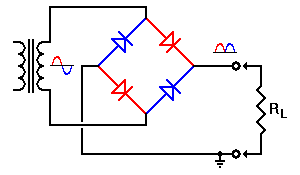
\includegraphics[width=0.8\textwidth]{images/bridgerectifier.png}\\
	Bridge Rectifier~\cite{rectifier}
\end{center}

\end{frame}



\begin{frame}
\frametitle{Rectification}

Rectification is a remedy of equity (fairness): it modifies the written document to express the real intentions of the parties.

It requires the following three conditions~\cite{lba}:

\begin{enumerate}
	\item A completed unambiguous contract that clearly expressed intentions.
	\item No change in the agreement between completion and writing it down.
	\item Evidence to convince the court that it contains a mistake such that the contract does not reflect the terms of the agreement.
\end{enumerate}

The onus is on the plaintiff to prove the third point.

\end{frame}


\begin{frame}
\frametitle{More Common Errors}

In the case of \textit{Couturier v. Hastie}, 1856~\cite{lba}, the parties arranged for the sale of corn en route from Thessaloniki, Greece to England.

Unknown to both parties, the cargo overheated and was in danger of spoiling.

The ship arrived at Tunis (Tunisia) and sold the corn.

The seller brought an action to recover the agreed price for the cargo.

Will Couturier succeed?

\end{frame}



\begin{frame}
\frametitle{Expiration}

No - the contract was held to be void.

Both parties made a common mistake, assuming that the goods existed and had not perished (``gone bad'').

Without the knowledge of either party, the goods being sold had ceased to exist (or be available for sale) and therefore a contract could not have been formed.

\end{frame}



\begin{frame}
\frametitle{I Come From a Land Down Under}

An Australian case: \textit{McRae v. Commonwealth Disposals Commission}, 1951.

The commission sold McRae a shipwrecked tanker containing oil.

The shipwreck, however, did not exist.

In this case, the CDC had claimed that the contract was void because it was a common mistake.

The court disagreed. Why?

\end{frame}



\begin{frame}
\frametitle{I Come From a Land Down Under}

The court found that CDC had promised the tanker existed. 

The \textit{Couturier v. Hastie} precedent was the seller suing the buyer for goods that the seller was unable to deliver.

Now it is the buyer suing the seller for representing the existence of a tanker when no such tanker ever existed.

Thus, CDC breached\footnote{Breach of Contract will be a major topic soon} the contract and owed damages to the buyer.

\end{frame}



\begin{frame}
\frametitle{Another Mistake}
\textit{Great Peace Shipping Ltd v Tsavliris Salvage(International) Ltd.,} 2002.

Tsavliris was in the business of aiding and salvaging ships.

The \textit{Cape Providence} required assistance and Tsavliris was told the tug \textit{Great Peace} was 35 miles away.

Tsavliris entered into a contract, but terminated it later when he determined the tug was 410 miles away.

There is a mistake here; does it render the contract void or voidable?

\end{frame}



\begin{frame}
\frametitle{Another Mistake}

No. Although the ship was about 10 times farther away than thought...

It would take about 22 hours to cover that distance, but the delay was not sufficiently large that it substantially redefined the contract.

The court said it would not be ``essentially different from those the parties envisaged when the contract was concluded.''


\end{frame}



\begin{frame}
\frametitle{Mutual Mistake}

Despite the confusing name, mutual mistake is distinct from common mistake.

In a mutual mistake situation, the parties think they are agreeing, but they mean different things. 

Case: \textit{Raffles v. Wichelhaus}, 1864.

\end{frame}




\begin{frame}
\frametitle{\textit{Raffles v. Wichelhaus}}

The parties entered into a contract stating the buyer would purchase cotton from Bombay.

It specified that the cotton would be coming on a ship called \textit{Peerless}.

Unfortunately, two ships with this name were coming from Bombay; one in October and one in December.

The buyer expected the cotton in October; it actually arrived in December.

What will the court do in this situation?

\end{frame}



\begin{frame}
\frametitle{Reasonable Interpretation}

The court will try to come up with a reasonable interpretation.

Given the misunderstanding, the courts will ask what interpretation of the contract makes the most sense.

If they are unable to do so, then the contract will be declared void.

What happened in the \textit{Raffles v. Wichelhaus} case?

\end{frame}



\begin{frame}
\frametitle{We Give Up}

In this example the court found no agreement on what a reasonable interpretation of the contract would be.

Which ship called \textit{Peerless} was the one named in the contract?

Thus the court found that there was no meeting of the minds and the contract, lacking this essential element, was void.


\end{frame}



\begin{frame}
\frametitle{Alternative Example}

Here, a case where the court could determine what a reasonable person would have thought: \textit{Lindsey v. Heron}~\cite{lba}.

The seller asked the buyer for a price for the purchase shares of a company ``Eastern Cafeterias of Canada.''

The buyer said he would buy shares of ``Eastern Cafeterias'' at \$10.50/share.

The seller sent the shares and the buyer sent a cheque.

Later the buyer realized that ``Eastern Cafeterias'' and ``Eastern Cafeterias of Canada'' were two different companies (and he meant the former!).

The court found that a reasonable person would have understood ``Eastern Cafeterias of Canada'' because the seller was unambiguous in the first place.

\end{frame}



\begin{frame}
\frametitle{Unilateral Mistakes}

Unilateral mistakes arise when only one party has made a mistake. 

Remember: the other party must know the first party made a mistake.

There are three major categories of unilateral mistake:

\begin{enumerate}
	\item About an essential term
	\item About the identity of a party 
	\item About the nature of a signed document
\end{enumerate}

We will skip over items 2 \& 3 in our discussion; while interesting for lawyers they are a bit beyond what we will cover in this course.

Item 1 is most relevant in engineering in the case of bids with errors in them.

\end{frame}



\begin{frame}
\frametitle{\textit{Hartog v Colin \& Shields}, 1939}

It was agreed that 30,000 hare skins would be sold at 10 d per skin $\rightarrow$ \textsterling1 250.

The written contract, however, said ``30,000 skins @ 10 d per lb''.

This reduced the amount to approximately \textsterling400 -- less than a third.

Obviously, the defendant made an error (about an essential term). 

Did the plaintiff know? What if the plaintiff did not know?

\end{frame}


\begin{frame}
\frametitle{\textit{Hartog v Colin \& Shields}, 1939}

The courts found: the plaintiff must have known the defendant made an error.\\
\quad And it was wrong to take advantage of that error.

The court can find a party knew something based on direct or indirect evidence.

There is also the ``reasonable person'' standard.

Thus it is sufficient if a party ``knew or ought reasonably to have known...''

(What would a reasonable person have known under the circumstances?)

\end{frame}


\begin{frame}
\frametitle{\textit{Imperial Glass Ltd. v Consolidated Supplies Ltd.}}

After receiving the dimensions of a window over the phone, an employee of the defendant calculated 202.62 sq. ft. instead of 2026.24 sq. ft. 

This resulted in a quote for \$2000.

Based on this number, the appellant submitted a bid.

Further communications included:

\begin{quote}
		We confirm herewith our quotation of \$2,000.00 for supplying the 	following Twin-Seal Units for Kitimat Elementary School.
\end{quote}

\begin{quote}
		It is to be understood that the above quotation is based on the 	number of units and sizes as indicated and any changes will call for 	a revision of this quotation.
\end{quote}

The order was placed; the defendant attempted to withdraw from the contract.\\
\quad What did the court do?

\end{frame}




\begin{frame}
\frametitle{\textit{Imperial Glass Ltd. v Consolidated Supplies Ltd.}}

The court determined that the behaviour of the plaintiff was seriously unethical, but not fraud.

The contractor was unaware of the error at the time of singing the contract.

The court did not relieve the defendant for their mistake.

\end{frame}



\begin{frame}
\frametitle{Other Precedent}

There is another case about a mistake in a contract:
\textit{Belle River Community Arena Inc. v W.J.C. Kaufmann Co. et al}.

This case drew a subsequent distinction about what was a mistake, but we will need to return to this in our later discussion of tendering.

Similarly, there is also the famous \textit{R. v. Ron Engineering \& Construction (Eastern) Ltd.} which is also about tendering.


\end{frame}


\begin{frame}
\frametitle{References \& Disclaimer}
\bibliographystyle{alphaurl}
\setbeamertemplate{bibliography item}{\insertbiblabel}
{\scriptsize
\bibliography{290}
}
\vfill

{\tiny Disclaimer: the material presented in these lectures slides is intended for use in the course ECE~290 at the University of Waterloo and should not be relied upon as legal advice. Any reliance on these course slides by any party for any other purpose are the responsibility of such parties.  The author(s) accept(s) no responsibility for damages, if any, suffered by any party as a result of decisions made or actions based on these course slides for any other purpose than that for which it was intended.\par}


\end{frame}


\end{document}

